\documentclass[tikz,border=3pt]{standalone}
\usepackage{fontspec}
\IfFontExistsTF{Times New Roman}
  {\setmainfont{Times New Roman}}
  {\setmainfont{TeX Gyre Termes}}
\usepackage{amsmath,amssymb}
\usepackage{xcolor}
\usepackage{tikz}
\usetikzlibrary{arrows.meta,positioning,calc,fit,backgrounds,shapes.geometric,decorations.pathreplacing,pgfplots.groupplots}
\definecolor{QFlowNavy}{HTML}{17365D}
\definecolor{QFlowBlue}{HTML}{2F5597}
\definecolor{QFlowTeal}{HTML}{2A7F7F}
\definecolor{QFlowAmber}{HTML}{8B5A00}
\definecolor{QFlowGray}{HTML}{667085}
\definecolor{QFlowLine}{HTML}{CBD5E1}
\definecolor{QFlowPaleBlue}{HTML}{EAF1F8}
\definecolor{QFlowPaleGray}{HTML}{F2F4F7}
\tikzset{
  qbox/.style={draw=QFlowNavy,rounded corners=1.2mm,fill=white,
    line width=0.6pt,align=center,inner sep=2.2mm,font=\fontsize{8.5}{10}\selectfont},
  qsoft/.style={qbox,fill=QFlowPaleBlue},
  qoutside/.style={qbox,draw=QFlowGray,dashed,fill=QFlowPaleGray},
  qarrow/.style={-{Latex[length=2mm,width=1.3mm]},line width=0.7pt,QFlowNavy},
  qdasharrow/.style={qarrow,dashed,QFlowGray},
  qlabel/.style={font=\fontsize{8}{9.2}\selectfont,align=center},
  qsmall/.style={font=\fontsize{7.5}{8.7}\selectfont,align=center}
}

\begin{document}
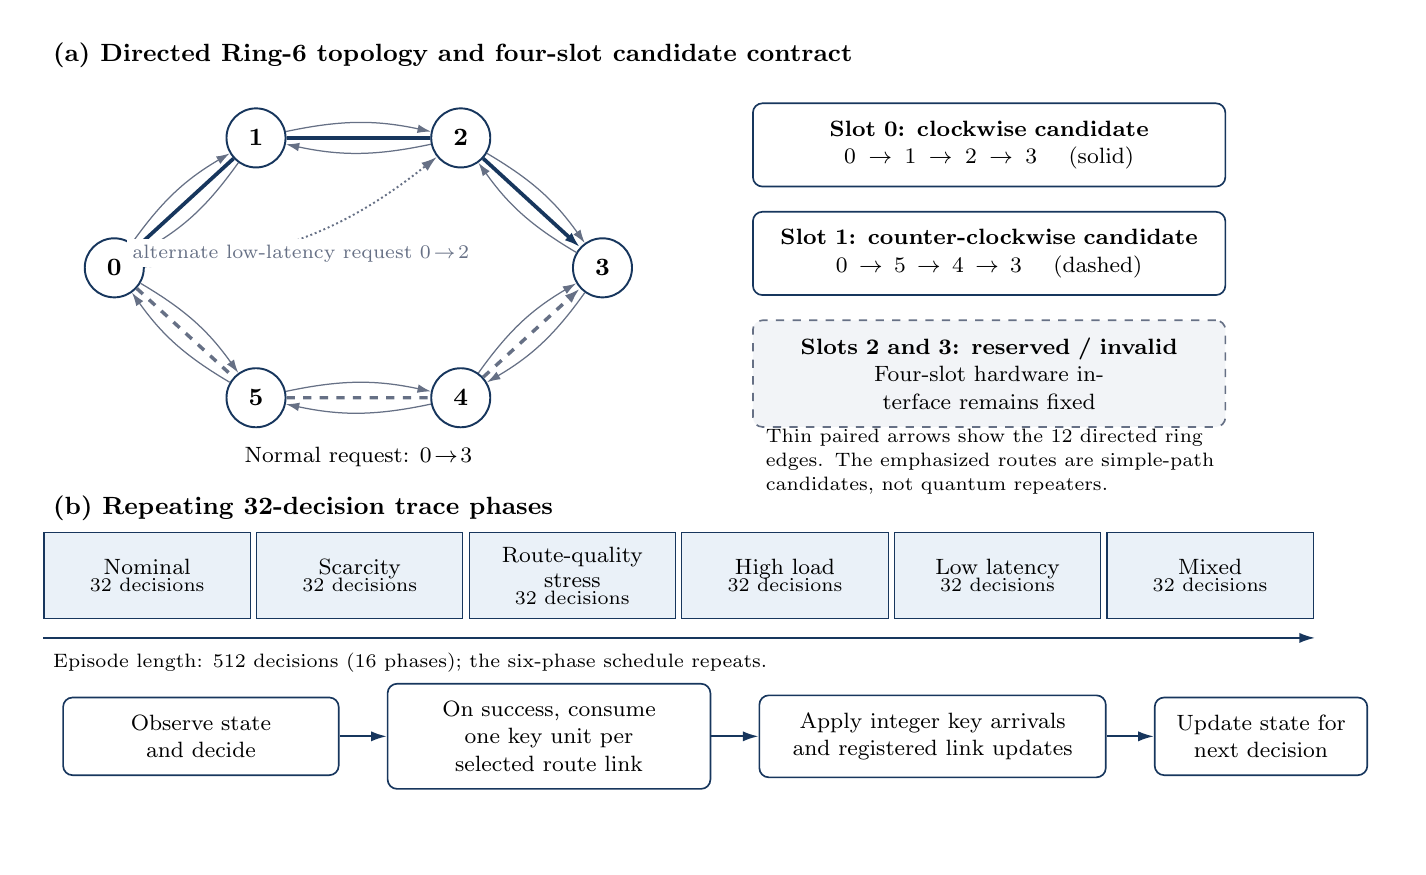
\begin{tikzpicture}[x=1cm,y=1cm]
  \path[use as bounding box] (-0.2,-5.25) rectangle (17.2,5.15);
  \tikzset{
    ringnode/.style={circle,draw=QFlowNavy,fill=white,minimum size=7.5mm,
      line width=0.7pt,font=\fontsize{9}{10}\selectfont\bfseries},
    baseedge/.style={-{Latex[length=1.7mm,width=1.1mm]},QFlowGray,line width=0.45pt},
    slot/.style={qbox,minimum width=6.0cm,text width=5.5cm,minimum height=8mm},
    phase/.style={draw=QFlowNavy,fill=QFlowPaleBlue,minimum width=2.62cm,
      minimum height=11mm,align=center,font=\fontsize{7.8}{9}\selectfont}
  }

  \node[qlabel,anchor=west,font=\fontsize{9}{10.5}\selectfont\bfseries] at (0,4.8)
    {(a) Directed Ring-6 topology and four-slot candidate contract};
  \node[ringnode] (n0) at (0.9,2.1) {0};
  \node[ringnode] (n1) at (2.7,3.75) {1};
  \node[ringnode] (n2) at (5.3,3.75) {2};
  \node[ringnode] (n3) at (7.1,2.1) {3};
  \node[ringnode] (n4) at (5.3,0.45) {4};
  \node[ringnode] (n5) at (2.7,0.45) {5};

  \foreach \a/\b in {n0/n1,n1/n2,n2/n3,n3/n4,n4/n5,n5/n0}{
    \draw[baseedge] (\a) to[bend left=12] (\b);
    \draw[baseedge] (\b) to[bend left=12] (\a);
  }
  \draw[qarrow,line width=1.35pt] (n0)--(n1)--(n2)--(n3);
  \draw[qdasharrow,line width=1.25pt] (n0)--(n5)--(n4)--(n3);
  \draw[qdasharrow,densely dotted,bend right=18] (n0) to node[qsmall,below,fill=white,inner sep=0.7mm]
    {alternate low-latency request $0\!\rightarrow\!2$} (n2);
  \node[qlabel,anchor=north] at (4.0,-0.05)
    {Normal request: $0\!\rightarrow\!3$};

  \node[slot,anchor=north west] (s0) at (9.0,4.2)
    {\textbf{Slot 0: clockwise candidate}\\$0\!\rightarrow\!1\!\rightarrow\!2\!\rightarrow\!3$ \quad (solid)};
  \node[slot,anchor=north west,below=3mm of s0] (s1)
    {\textbf{Slot 1: counter-clockwise candidate}\\$0\!\rightarrow\!5\!\rightarrow\!4\!\rightarrow\!3$ \quad (dashed)};
  \node[qoutside,minimum width=6.0cm,text width=5.5cm,anchor=north west,below=3mm of s1] (s23)
    {\textbf{Slots 2 and 3: reserved / invalid}\\Four-slot hardware interface remains fixed};
  \node[qsmall,anchor=north west,text width=5.9cm,align=left] at (9.05,0.18)
    {Thin paired arrows show the 12 directed ring edges. The emphasized routes are simple-path candidates, not quantum repeaters.};

  \node[qlabel,anchor=west,font=\fontsize{9}{10.5}\selectfont\bfseries] at (0,-0.95)
    {(b) Repeating 32-decision trace phases};
  \foreach \x/\name in {0/Nominal,2.7/Scarcity,5.4/Route-quality\\stress,8.1/High load,10.8/Low latency,13.5/Mixed}{
    \node[phase,anchor=north west] at (\x,-1.25) {\name\\[-1mm]{\fontsize{7}{8}\selectfont 32 decisions}};
  }
  \draw[qarrow] (0,-2.6)--(16.15,-2.6);
  \node[qsmall,anchor=west,fill=white] at (0,-2.92)
    {Episode length: 512 decisions (16 phases); the six-phase schedule repeats.};

  \node[qbox,minimum width=3.5cm,text width=3.0cm] (decide) at (2.0,-3.85)
    {Observe state and decide};
  \node[qbox,minimum width=4.1cm,text width=3.6cm,right=6mm of decide] (consume)
    {On success, consume one key unit per selected route link};
  \node[qbox,minimum width=4.4cm,text width=3.9cm,right=6mm of consume] (update)
    {Apply integer key arrivals and registered link updates};
  \node[qbox,minimum width=2.7cm,text width=2.2cm,right=6mm of update] (next)
    {Update state for next decision};
  \draw[qarrow] (decide)--(consume);
  \draw[qarrow] (consume)--(update);
  \draw[qarrow] (update)--(next);
\end{tikzpicture}
\end{document}
